\documentclass[12pt]{aghdpl}
% \documentclass[en,11pt]{aghdpl}  % praca w języku angielskim
\usepackage[polish]{babel}
%\usepackage[english]{babel}
\usepackage[utf8]{inputenc}
\usepackage{url}
\usepackage[usenames,dvipsnames,svgnames,table]{xcolor}

% dodatkowe pakiety
\usepackage{enumerate}
\usepackage{listings}
\usepackage{amsmath}
\usepackage{algorithm2e}
\usepackage{fixltx2e}
\usepackage{subcaption}
\usepackage[section]{placeins}
\lstloadlanguages{TeX}

\lstset{
  literate={ą}{{\k{a}}}1
           {ć}{{\'c}}1
           {ę}{{\k{e}}}1
           {ó}{{\'o}}1
           {ń}{{\'n}}1
           {ł}{{\l{}}}1
           {ś}{{\'s}}1
           {ź}{{\'z}}1
           {ż}{{\.z}}1
           {Ą}{{\k{A}}}1
           {Ć}{{\'C}}1
           {Ę}{{\k{E}}}1
           {Ó}{{\'O}}1
           {Ń}{{\'N}}1
           {Ł}{{\L{}}}1
           {Ś}{{\'S}}1
           {Ź}{{\'Z}}1
           {Ż}{{\.Z}}1
}

%---------------------------------------------------------------------------

\author{Agata Paciorek}
\shortauthor{A. Paciorek}

\titlePL{Segmentacja obiektów pierwszoplanowych w warunkach obecności drobnego ruchu na scenie}
\titleEN{Foreground object segmentation in presence of background clutter}

\shorttitlePL{Segmentacja obiektów pierwszoplanowych...} % skrócona wersja tytułu jeśli jest bardzo długi
\shorttitleEN{Segmentation}

\thesistype{Praca dyplomowa inżynierska}
%\thesistype{Master of Science Thesis}

\supervisor{dr inż. Tomasz Kryjak}
%\supervisor{dr inż. Tomasz Kryjak}

\degreeprogramme{Informatyka}
%\degreeprogramme{Computer Science}

\date{2015}

\department{Katedra Automatyki i Inżynierii Biomedycznej}
%\department{Department of Automatics and Biomedical Engineering}

\faculty{Wydział Elektrotechniki, Automatyki,\protect\\[-1mm] Informatyki i Inżynierii Biomedycznej}
%\faculty{Faculty of Electrical Engineering, Automatics, Computer Science and Biomedical Engineering}

\acknowledgements{Serdecznie dziękuję %doktorowi Tomaszowi Kryjakowi za nadzór nad procesem tworzenia pracy \\
%oraz \\
%Michałowi Drobniakowi - za wsparcie.
}


\setlength{\cftsecnumwidth}{10mm}

%---------------------------------------------------------------------------

\begin{document}

\titlepages

\tableofcontents
\clearpage

\chapter{Wstęp}
\label{cha:wstęp}

\paragraph{}
Ilość generowanej przez człowieka informacji w ostatnich latach gwałtownie wzrasta. Dynamiczny rozwój  Internetu i szeroko pojętej technologii  oraz wzrost jej dostępności na niemal całym świecie spowodował, iż o wiele prościej jest zarówno pozyskiwać wiedzę, jak i dzielić się nią. W przeciągu ostatnich czterdziestu lat, od czasu pojawienia się sieci komputerowej, poszerzyły się także możliwości przechowywania danych. Miniaturyzacja urządzeń wraz ze wzrostem jakości pozyskiwanych informacji sprzyjają coraz dalszemu rozwojowi technologii informacyjnej. Dlatego też tak ważna jest automatyzacja procesów analizy informacji, bez której pozyskiwanie istotnych faktów byłoby bardzo utrudnione, jeżeli nie niemożliwe. 
\paragraph{}
Jedną z dziedzin, która doświadcza ciągłego rozwoju, jest monitoring wizyjny. W większych miastach na kamery monitorujące można natknąć się nieomal na każdym kroku - począwszy od budynków, takich jak biurowce, strzeżone osiedla czy szkoły, po zintegrowane systemy monitoringu całego miasta. Można się spotkać nawet z monitoringiem podwodnym. Coraz wyższa jakość pozyskiwanego z kamer obrazu oraz wzrastająca liczba montowanych urządzeń powoduje, iż objętość danych uzyskiwanych w ten sposób nie przestaje się powiększać. Dlatego też monitoring oparty na analizie bieżącego materiału wideo przez człowieka staje się w dużej mierze niewystarczający.
\paragraph{}
Ograniczenia percepcji ludzkiego ciała powodują, iż w wielu przypadkach maszyny zaczynają przewyższać możliwości ludzi. Ciągłe skupianie uwagi na analizie obserwowanej przez operatora sceny może prowadzić do znużenia i wolniejszej detekcji ewentualnego zagrożenia. Nie bez znaczenia jest również fakt, iż kiedy na nagraniu nie ma wartkiej akcji - a tak zdarza się nieczęsto - uwaga obserwatora z czasem spada. Rzadko również zdarza się, że pracownik ma do czynienia z obrazem tylko z jednej kamery - najczęściej jest to kilka nagrań, wyświetlanych na osobnych urządzeniach, bądź na jednym monitorze z możliwością przełączania się między scenami. W obu przypadkach człowiek boryka się z ograniczeniami dotyczącymi równoczesnej analizy wielu scen. Czynniki te, u człowieka powodujące zmniejszoną zdolność percepcji, maszyn nie dotyczą. Mogą one zatem pomóc w uzyskaniu z obrazów istotnej informacji.
\paragraph{}
Abstrahując od hipotetycznej możliwości całkowitego zastąpienia człowieka maszyną w kwestii obserwacji i analizy obrazów, już samo wykrycie przez odpowiedni system zmian na scenie i zasygnalizowanie ich operatorowi znacznie zwiększa prawdopodobieństwo wykrycia nieprawidłowości. Możliwości obliczeniowe obecnych maszyn, ze szczególnym uwzględnieniem czasu wykonywania operacji, są powodem, dla którego empiryczne postrzeganie świata przez człowieka da się zastąpić właśnie odpowiednim systemem komputerowym. Twórcy oprogramowania takich systemów borykają się jednak z wieloma problemami. Jednym z nich jest prawidłowa segmentacja obiektów pierwszoplanowych, o której będzie mowa w tej pracy. Polega ona na wyodrębnieniu elementów sceny niosących istotną informację i nie należących do tła, jak choćby pieszych, samochodów czy innych pojazdów. Tak uzyskane wyniki mogą być dowolnie przetwarzane, co umożliwia na przykład badanie zachowania ludzi w celu wykrycia niebezpiecznych sytuacji czy informowanie o obiektach pozostawionych na scenie, potencjalnie również stwarzających zagrożenie - na przykład plecak porzucony na dworcu kolejowym może zawierać ładunek wybuchowy. Segmentacja ta nie jest jednak zagadnieniem prostym - przeważnie system ma do czynienia z prawdziwymi nagraniami, na których ''sterylne'' warunki (niezmienne warunki oświetleniowe/pogodowe, statyczne tło) występują bardzo rzadko. Jednym z wyzwań jest kwestia wyeliminowania detekcji drobnego ruchu sceny, nieistotnego z punktu niesionej przez niego informacji - takiego jak nieznaczne drgania liści na wietrze, czy zmienne refleksy świetlne w wodzie płynącej w fontannie bądź innych zbiornikach wodnych. Bardzo rzadko zdarza się, iż na monitorowanej na zewnątrz budynku scenie nie występuje żadne z tych zjawisk, dlatego tak ważne jest rozwiązanie problemu. Standardowe podejścia w detekcji ruchu nie umożliwiają odseparowania takich drobnych poruszeń od większych zmian na nagraniu, segmentacja obiektów pierwszoplanowych przy ich pomocy często prowadzi więc do błędnych wyników.

%---------------------------------------------------------------------------

\section{Cele pracy}
\label{sec:celePracy}

Celem niniejszej pracy jest przeanalizowanie kilku dostępnych już udokumentowanych rozwiązań i\,zaproponowanie najlepiej sprawdzającego się z nich sposobu segmentacji obiektów pierwszoplanowych przy obecności drobnego ruchu na scenie. Zaimplementowane zostaną odpowiednie algorytmy oraz zbadane będą ich możliwości w kwestii szybkości i dokładności detekcji. 


%---------------------------------------------------------------------------

\section{Zawartość pracy}
\label{sec:zawartoscPracy}

W rodziale~\ref{cha:analiza} przedstawiono dostępne na rynku algorytmy. 



















\chapter{Wprowadzenie do tematyki pracy}
\label{cha:tematykaPracy}
Cyfrowa akwizycja obrazu pozwala na odwzorowanie widzialnej dla człowieka sceny w przestrzeni zdigitalizowanej. Takie przedstawienie obrazu umożliwia utrwalenie go na rozmaitych nośnikach pamięci i dostęp do niego w dowolnym momencie w przyszłości. Rejestrując zdjęcia z pewną częstotliwością i zachowaniem kolejności ich akwizycji otrzymuje się nagranie wideo. Pozwala ono śledzić zmiany na scenie następujące w czasie, takie jak ruch czy \textcolor{red}{zmiana} oświetlenia. Następujące po sobie obrazy zwane \textbf{ramkami} to \textbf{sekwencja wideo}.
\section{Preprocessing}
Choć dla człowieka informacje zawarte na obrazie są proste w interpretacji, maszyna ''widzi'' ramkę jako zwykły ciąg liczb. Dlatego aby dokonywać automatycznej detekcji pewnych zjawisk i zależności, należy poddać ją odpowiednim przekształceniom, pozwalającym wyekstrahować interesujące powiązania. Zanim jednak to się stanie, należy między innymi dokonać uwydatnienia pożądanych cech na obrazie i pozbyć się zakłóceń, czyli poddać go filtracji. Taki proces nazywa się przetwarzaniem wstępnym, czyli \textit{preprocessingiem}. Do tej fazy wliczamy m.in.:
\begin{itemize}
\item przekształcenia geometryczne, wykorzystywane do korekcji błędów urządzeń akwizycyjnych
\item przekształcenia punktowe, nie wymagające znajomości otoczenia piksela
\item przekształcenia kontekstowe - na przykład filtry, ustalające wartość piksela na podstawie poziomu jasności pikseli z nim sąsiadujących
\item przekształcenia widmowe, jak  np. transformata Fouriera
\item przekształcenia morfologiczne, modyfikujące wartość piksela przy spełnieniu pewnego warunku logicznego
\end{itemize}
W zależności od tego, jakie elementy ramki są w programie istotne, stosuje się różne metody uwydatnienia informacji. W książce \cite{i1823330731}, z której pochodzi wspomniana wyżej klasyfikacja, opisane są najczęściej wykorzystywane algorytmy używane w takim procesie. W tej sekcji zostaną przedstawione niektóre z nich, istotne w kontekście niniejszej pracy.
\subsection{Filtracja}
Filtracja obrazu ma na celu wyeliminowanie niepożądanych cech obrazu. Jest to operacja kontekstowa, a więc wymagająca informacji o jasności piksela i jego otoczenia. Staje się przez to procesem wykorzystującym duże nakłady obliczeniowe maszyny, przez co znacznie opóźnia działanie metody wykorzystującej filtrację - dlatego też istotny jest dobór jak najbardziej optymalnego sposobu eliminacji zakłóceń w zależności od danych. Dostępnych jest wiele metod, jak choćby filtracja górno- lub dolnoprzepustowa czy filtracja medianowa. Dokonuje się także klasyfikacji filtrów na liniowe (w oparciu o kombinację wartości odpowiednich pikseli obrazu wejściowego) i nieliniowe (do przekształceń wykorzystujące nieliniową funkcję odpowiednich pikseli obrazu). 
\subsubsection{Konwolucja}
Operacją wykorzystywaną przy filtrach liniowych jest splot funkcji, czyli konwolucja. Ponieważ reprezentacja obrazów w przestrzeni cyfrowej jest dyskretna, również operacja splotu, w przestrzeni liczb rzeczywistych definiowana jako całka, może być opisana za pomocą zwykłego równania sumy:
\begin{equation}
\label{eq:konwolucja}
L'(m,n) = (w x L)(m,n) = \sum_{i,j \in K} L(m-i, n-j)w(i,j)
\end{equation}
, gdzie L - obraz wejściowy, L' - efekt splotu obrazu z maską konwolucji, w - maska konwolucji, (m, n) - współrzędne piksela, dla którego wykonywana jest konwolucja jego otoczenia z maską w.\\
Przykładowy splot fragmentu obrazu z maską filtru uśredniającego 3x3:
%\begin{equation}
\label{eq:konwolucjaPrzyklad}
\[
\begin{bmatrix}
    10 & 30  & 4 \\
    20 & \textcolor{red}{0}   & 5 \\
    0  & \textcolor{red}{100} & 102 \\
    20 & 50  & 20
\end{bmatrix}
\mathrm{x}
\begin{bmatrix}
    1 & 1 & 1 \\
    1 & 1 & 1 \\
    1 & 1 & 1
\end{bmatrix}
=
\begin{bmatrix}
    x &  x  & x \\
    x & 271 & x \\
    x & 317 & x \\
    x &  x  & x 
\end{bmatrix}
\]
%\end{equation}
\subsubsection{Normalizacja}
Ponieważ w konwolucji wykonywane są operacje mnożenia i dodawania, otrzymane wartości mogą znacznie wykraczać poza zakres, jaki należy uzyskać w danej przestrzeni - najczęściej powinna być to liczba z przedziału [0, 255]. Jak łatwo zauważyć, w przykładzie \ref{eq:konwolucjaPrzyklad} tak właśnie się stało. W celu dostosowania uzyskanych liczb do wymaganego zakresu dokonuje się normalizacji. Jeśli w masce obecne są wyłącznie elementy nieujemne, każdy wynik konwolucji dzielony jest przez sumę jej elementów. Jeśli jednak współczynniki w macierzy w są zarówno dodatnie, jak i ujemne, normalizacja musi odbywać się według następującego wzoru:
\begin{equation}
L''(m,n) = \dfrac{L'(m,n)-minL'(m,n)}{maxL'(m,n)-minL'(m,n)}
\end{equation}
\subsection{Przestrzenie barw}
\label{sec:colorSpace}
Przestrzeń barw to pewna matematyczna reprezentacja światła widzialnego w przestrzeni cyfrowej. W zależności od potrzeb stosowane są różne modele. Najpopularniejszymi są spotykane w urządzeniach elektronicznych trójkanałowe RGB (ang. \textit{Red Green Blue}) oraz komplementarny do niego, stosowany w druku CMYK (ang. \textit{Cyan Magenta Yellow blacK}), wykorzystujące właściwości ludzkiego wzroku determinujące sposób, w jaki człowiek odbiera barwy. Każdemu pikselowi obrazu są tu przypisane odpowiednie wartości na każdym kanale, na przykład czerwony piksel w reprezentacji RGB na kanale czerwonym (R) ma maksymalną wartość 255 (w 8-bitowej głębi kolorów), na niebieskim i zielonym po 0. Stosowane są one do łatwej do interpretacji przez człowieka reprezentacji cyfrowej kolorów na zdjęciach. Wprowadzają one jednak duże ograniczenia ze względu na ilość niesionej informacji. Akwizycja obrazu w innej przestrzeni pozwala na przykład na zastosowanie o wiele szerszego spektrum barw. Dlatego też często przy przetwarzaniu obrazów stosuje się inne modele, rozdzielające istotne dla maszyny informacje na oddzielne kanały, co umożliwia wydajniejsze i niekiedy dokładniejsze obliczenia na zdjęciach.
\paragraph{}
\begin{figure}[!htb]
\centering
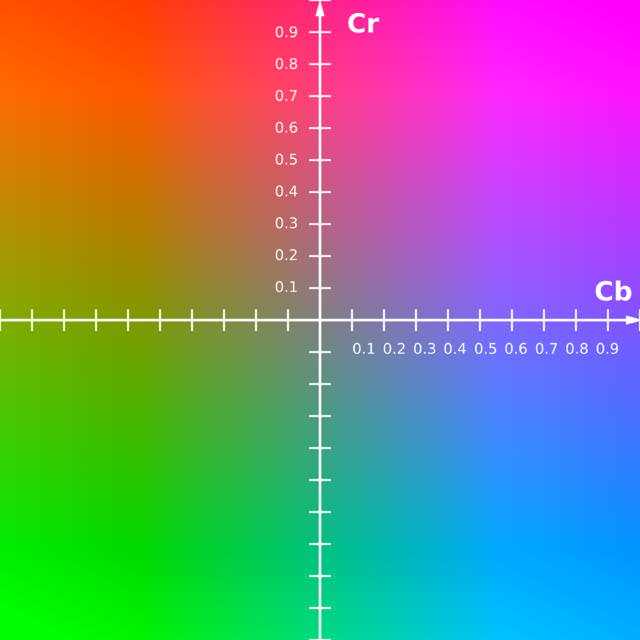
\includegraphics[width=182px]{img/YCbCr}
\caption{Reprezentacja płaszczyzny 
CbCr dla stałej luminancji Y=0.5}
%\floatfoot{Source: Wikipedia}
\end{figure}
W metodzie opisanej w rozdziale \ref{sec:BinWang}  używana jest przestrzeń YCbCr, oddzielająca kanał luminancji (Y), czyli poziomu jasności piksela, od kanałów chrominancji (Cb i Cr), przechowujących informację o jego odcieniu i nasyceniu. Taki sposób reprezentacji powstał z wykorzystaniem faktu, iż oko ludzkie jest o wiele bardziej czułe na poziom jasności obiektu, niż na jego kolor. Konwersja z przestrzeni RGB do YCbCr jest stosunkowo prosta - można ją zapisać w postaci macierzy:
%\begin{equation}

\[
\begin{bmatrix}
    Y & Cb & Cr \\
\end{bmatrix}
=
\begin{bmatrix}
    R & G & B \\
\end{bmatrix}
\begin{bmatrix}
    0.299 & -0.168935 & 0.499813 \\
    0.587 & -0.331665 & -0.418531 \\
    0.114 & 0.50059 & -0.081282 
\end{bmatrix}
\]

%\end{equation}

Ponieważ wartości na kanałach RGB mieszczą się w przedziale 0-255, po przekształceniu do przestrzeni YCbCr otrzymujemy odpowiednio wartości z przedziału [0, 255] na kanale Y oraz [-128, 127] na kanałach Cb i Cr.
\section{Analiza obrazu}  
\subsection{Binaryzacja}
Jest to jedna z podstawowych metod punktowego przetwarzania obrazu.  Pozwala odseparować istotne informacje na zdjęciu z pominięciem zależności mniej interesujących, takich jak na przykład konkretny poziom jasności, utrudniających tylko dalsze przetwarzanie ze względu na większą złożoność obliczeń. Obraz zostaje sprowadzony do postaci binarnej (zero-jedynkowej), gdzie najczęściej (w zależności od podejścia) 0 reprezentuje tło, 1 - interesujący obszar obrazu.  
\paragraph{}
Istnieje wiele metod binaryzacji, dlatego też można wybrać odpowiednią dla każdego algorytmu. Podstawowym problemem staje się jednak wyznaczenie odpowiedniego progu binaryzacji - ze względu na następującą w procesie radykalną redukcję informacji zawartych w obrazie, źle dobrany graniczny poziom jasności może doprowadzić do błędnej detekcji, w konsekwencji skutkującej złym działaniem programu. Dlatego też bardzo ważna jest znajomość rodzaju danych, z jakimi system przetwarzający będzie miał do czynienia - pozwoli to zastosować odpowiednią dla nich metodę obliczenia progu.
\subsection{Segmentacja obiektów}
Po dokonaniu binaryzacji otrzymujemy obraz czarno-biały, jednak wciąż konieczne jest przygotowanie uzyskanych wyników do dalszej analizy. Służy do tego metoda zwana segmentacją obrazu, polegająca na podziale obrazu na segmenty odpowiadające konkretnym utrwalonym na nim elementom.
\section{Detekcja ruchu na scenie}
Detekcja ruchu, czyli \textit{Motion Detection}, to sposób wykrywania przemieszczania się obiektów na scenie względem ich sąsiedztwa. Polega ona na analizie kolejnych ramek z sekwencji wideo i badaniu zmian następujących pomiędzy nimi.
\paragraph{}
Ze względu na trudność problemu detekcji, opracowanych zostało wiele metod odseparowania obiektów poruszających się od statycznych elementów sceny. Jedną z nich, stosunkowo najprostszą, jest odjęcie od obrazu wejściowego modelu uzyskanego przy pomocy algorytmów generacji tła. Na tym etapie twórcy metod muszą rozważyć jednak trzy podstawowe kwestie:
\begin{itemize}
\item czym jest model i jak się zachowuje?
\item jak dokonać inicjalizacji modelu tła?
\item w jaki sposób aktualizować model w czasie?
\end{itemize}
Związane jest to z faktem, iż bardzo rzadko na sekwencjach wideo rejestrowane są sytuacje idealne - często scenie towarzyszą zmiana oświetlenia (zwłaszcza w długotrwałym monitoringu na zewnątrz) lub szumy/zakłócenia, czego rezultatem jest, iż pomimo braku ruchu obiektów poszczególne piksele zmieniają swoją wartość - co przy standardowym podejściu polegającym na porównaniu wartości pikseli odpowiadających sobie pomiędzy ramkami skutkuje fałszywą detekcją. Rzadko również do dyspozycji są sekwencje z "czystym" obrazem tła - na próbkowanych ramkach znajdują obiekty już w ruchu, albo statyczne, jednak mogące w każdej chwili zmienić swoje położenie - jak choćby zaparkowane samochody. Zasłaniają one tło, przez do wygenerowanie prawidłowego modelu staje się bardzo trudne, a niekiedy niemożliwe. Opisane w dalszej części rozwiązania stworzone zostały z uwzględnieniem niniejszych ograniczeń.
\subsection{Modelowanie tła}
Jednym z najczęściej używanych w detekcji ruchu na scenie rozwiązań pośrednich jest modelowanie tła. Polega ono na stworzeniu modelu referencyjnego sceny bez żadnych ruchomych obiektów, co pozwala na późniejsze porównanie z nim kolejnych ramek nagrania w celu wykrycia zmian. Najczęściej odbywa się to poprzez algorytmy subtrakcji tła - obliczana jest absolutna różnica pomiędzy modelem tła a aktualnie analizowanym obrazem sceny, co skutkuje otrzymaniem obrazu, na którym niezerowe wartości są interpretowane jako obiekty pierwszoplanowe.
\paragraph{}
W rzeczywistości jednak to zagadnienie okazuje się być o wiele bardziej skomplikowane. W nagraniach rejestrowanych przez kamery w monitoringu wizyjnym rzadko dostępny jest materiał, na którym widoczne jest samo tło. Usuwanie wszelkich obiektów ze sceny i trenowanie maszyn monitorujących za każdym razem, kiedy tło zmieni się - na przykład zostanie wybudowany nowy budynek bądź nastąpi przemeblowanie wewnątrz pomieszczenia - jest bardzo uciążliwe. Twórcy oprogramowania zajmującego się automatyczną detekcją obiektów borykają się także z problemami, jakich nastręcza zjawisko ruchu obrotowego Ziemi - zmiennym oświetleniem sceny w zależności od pory dnia. Trzeba bowiem brać pod uwagę, iż na obrazie reprezentowana jest jasność poszczególnych pikseli - im mniej światła, tym ciemniejsze stają się obiekty. Można pomyśleć, iż ta kwestia rozwiązana zostać może poprzez zmianę przestrzeni kolorów i odseparowanie luminancji pikseli od ich barwy (\ref{sec:colorSpace}), jednak i tu pojawiają się problemy - mniej światła oznacza dużo mniej dokładną akwizycję barwy piksela, a co za tym idzie mogą pojawiać się różnice odcieni w czasie. Występuje tu analogia do procesu widzenia człowieka - oko ludzkie potrafi rozpoznawać kształt i ruch nawet przy bardzo słabym oświetleniu, odbywa się to jednak kosztem postrzegania w kolorze. W półmroku człowiek rejestruje więc otoczenie w skali szarości.
\paragraph{}
Z tych i wielu innych powodów zagadnienie modelowania tła staje się kluczowym w przypadku wielu algorytmów. Dobry obiekt referencyjny pozwala bowiem na ograniczenie detekcji do zwykłego porównywania wartości poszczególnych pikseli. Najczęściej proces modelowania odbywa się na podstawie początkowej sekwencji testowej, a następnie wzorzec tła jest uaktualniany poprzez odpowiednie modyfikacje przez cały czas działania programu wykrywającego ruch. Stosowanych jest wiele podejść, wykorzystujących zarówno proste mechanizmy, jak średnia wartość piksela na obrazie, jak i nieco bardziej zaawansowane, oparte na statystyce i probabilistyce. Warto wspomnieć tu o modelach gaussowskich, pojawiających się w większości proponowanych obecnie rozwiązań. Zasada ich działania opisana zostanie w dalszej części pracy.
\paragraph{}
Standardowe podejścia w dziedzinie generacji tła, jak średnia jasność bądź model Gaussa na podstawie pojedynczej ramki, nie dają jednak spodziewanych rezultatów w przypadkach obecności drobnego ruchu na scenie. Obiekty tła pozostające w ciągłym \textcolor{red}{ruchu} mogą bowiem przyjmować diametralnie skrajne wartości jasności. Posiadanie więc jednego modelu tła okazuje się nie być wystarczające. Te same algorytmy dla różnych zestawów nagrań wykazują się odmienną skutecznością, co jest zjawiskiem niepożądanym - dobry system detekcji powinien pracować prawidłowo niezależnie od panujących warunków.
\begin{figure}[!htb]
\centering


\includegraphics[width=0.4\textwidth]{img/sample}

\includegraphics[width=0.4\textwidth]{img/sample}
\caption{Modelowanie tła. Po lewej - ramka z nagrania, po prawej wyidealizowany model tła}
%\floatfoot{Source: }
\end{figure}
\subsection{Metody uaktualniania modelu tła}
Aby utrzymać prawidłową pracę systemu detekcji w zmiennych warunkach, należy dokonywać uaktualniania modelu tła na bieżąco. Polega to na podmianie wartości niektórych pikseli modelu bardziej \textcolor{red}{aktualnymi}. Ze względu na politykę stosowaną w tym procesie wyróżniane są dwie metody:
\begin{itemize}
\item konserwatywna
\item ślepa
\end{itemize} 
Metoda \textbf{konserwatywna} (ang. \textit{conservative update}) polega na uaktualnianiu wartości tylko dla tych pikseli, które zaklasyfikowane zostały obecnie jako tło. Choć z pozoru najbardziej intuicyjna, może doprowadzić do poważnych problemów na przykład przy błędnej detekcji elementów tła - jeśli nieprawidłowo wykryto ruch, nie będzie możliwe uaktualnianie modelu dla fałszywie sklasyfikowanych pikseli. Prowadzi to do powstawania tak zwanych \textbf{duchów} (ang. \textit{ghosts}) - efektów błędnej detekcji, które są propagowane w dalszym procesie działaniu algorytmu. Alternatywą dla tego sposobu jest metoda \textbf{ślepa} (ang. \textit{blind update}). Choć zapobiega zakleszczeniom, które mogą zdarzyć się przy polityce konserwatywnej, daje bardzo słabe wyniki dla obiektów poruszających się wolno, jako że piksele uaktualniane są niezależnie od tego, do którego modelu zostały przydzielone.
\section{Standardowe metody detekcji ruchu na scenie}
\subsection{Średnia bieżąca}
Algorytm średniej bieżącej to bezparametrowa metoda detekcji ruchu oparta na zależnościach statystycznych. Polega ona na analizie rozkładu prawdopodobieństwa wystąpienia pewnych wartości jasności (koloru) piksela na podstawie jego sąsiedztwa.\\
\nocite{kheng2011mean}
Średnia bieżąca (ang. \textit{mean shift}) wyznaczana jest metodą iteracyjną dla każdej próbki obrazu oddzielnie. Dla danego piksela x oblicza się średnią tymczasową m(x) z jego otoczenia, która przedstawia się wzorem:
\begin{equation}
m(x) = 
\frac{\sum_{i=1}^{n}K(x-x_{i})x_{i}}{\sum_{i=1}^{n}K(x-x_{i})}
\end{equation}
, gdzie K - kernel, w którym zawarte są wagi, z jakimi brane są pod uwagę piksele sąsiedztwa x\textsubscript{i}, n - ilość pikseli sąsiedztwa \\
Średnią bieżącą nazywamy różnicę m(x) - x.
Następnie należy sprawdzić, czy wartość piksela równa jest średniej tymczasowej, czyli czy m(x) == x. Jeśli nie - należy przypisać x = m(x) i rozpocząć wyznaczanie średniej dla nowej wartości x. Jeśli jednak tak, algorytm kończy się.\\
Jeśli średnie tymczasowe obliczane są dla wielu punktów, aktualizacja ich wartości odbywa się równocześnie w każdej iteracji.
\paragraph{}
W ten sposób otrzymana średnia bieżąca może zostać użyta do wykrywania ruchu na scenie. Tworzona jest mapa gęstości prawdopodobieństwa na podstawie histogramu kolorów obiektu w poprzedniej ramce (dla każdego piksela osobno), a następnie wyszukuje się w niej szczytowej wartości w pobliżu wcześniejszego położenia obiektu. Pozwala to na wykrycie kierunku ruchu obiektu zmieniającego położenie.
\paragraph{}
Najczęściej wspominaną wadą takiego podejścia jest konieczność używania stałej wielkości ramki, w której ma znajdować się śledzony obiekt. Niewygodne staje się więc śledzenie obiektów zmieniających rozmiar w czasie, jak np. nadjeżdżających samochodów obserwowanych z odpowiedniej perspektywy. Bardziej elastyczną wersją tej metody jest CAMSHIFT (ang. \textit{Continuous Adaptive Mean Shift}, potrafiąca dostosować się do zmian w kolorystyce obiektu, a także jego rozmiarze. Implementacja obu algorytmów dostępna jest w bibliotece OpenCV.\\ \\ \\
\begin{LARGE}
\textcolor{red}{WYNIKI DLA DYNAMIC BG}
\end{LARGE}

\subsection{Gaussian Mixture Model}
\label{sec:GMM}
Metoda ta \cite{zivkovic2004improved} opiera się na obserwacji, iż obiekty tła, przy braku przemieszczających się obiektów na scenie, wykazują pewne zależności, które mogą zostać przedstawione za pomocą modeli statystycznych. Dlatego też wyodrębnienie pikseli nie pasujących do takiego modelu wiąże się z wykryciem ruchu na scenie. Jest to stosunkowo mało skomplikowany algorytm oparty na mechanizmie subtrakcji tła.
\paragraph{}
Pierwszym etapem działania algorytmu jest wyznaczenie modelu tła. Odbywa się to na podstawie gaussowskiego rozkładu prawdopodobieństwa dla każdego piksela sceny. Estymowane wartości modelu tła otrzymywane są w wyniku analizy określonej liczby próbek w czasie t. Następnie odbywa się klasyfikacja pikseli. Jeżeli prawdopodobieństwo wystąpienia danego piksela w ramce t+n jest większe od pewnego ustalonego progu, zostaje on sklasyfikowany jako tło. W przeciwnym wypadku przypisuje się go do modelu pierwszoplanowego.\\
Głównym problemem, z jakim spotyka się ta metoda, jest problem z adaptacją do zmian na scenie, na przykład w oświetleniu.\\
Prawdopodobieństwo wystąpienia danej wartości piksela x w ramce t przy K jako liczbie gausjanów używanych w modelu dane jest następującym wzorem:
\begin{equation}
P(x_{t}) = \sum_{i=1}^{K} waga_{i,t}*g(x_{t},\mu_{i,t},\sigma_{i,t})
\end{equation}
, gdzie g(a,b,c) - funkcja gęstości prawdopodobieństwa dla rozkładu Gaussa, $\mu$ - wartość średnia, $\sigma$ - odchylenie standardowe.\\
Głównym zagadnieniem dla tej metody jest kwestia doboru próbek, na podstawie których wyznaczane jest prawdopodobieństwo. Zbyt mała bądź źle dobrana ich ilość powoduje fałszywą detekcję w przypadku znacznej zmienności tła, zbyt duża - zawyżoną tolerancję, przez co piksele pierwszoplanowe zostają niekiedy sklasyfikowane jako tło.

\subsection{ViBE}
Autorzy pracy \cite{barnich2011vibe} zaproponowali jeszcze inny sposób na dokonywanie detekcji w zmieniających się warunkach otoczenia. Zamiast modelować i przewidywać wartość piksela, postanowili oni przechowywać informację o jego wcześniejszych reprezentacjach.
\paragraph{}
ViBE (ang. \textit{VIsual Background Extractor}) porzuca koncepcję estymacji pożądanej wartości piksela na podstawie wielu globalnych próbek, mogących zawierać wartości skrajnie odbiegające od średnich wartości. Zamiast tego skupia się na badaniu podobieństwa aktualnego piksela do wartości zarejestrowanych uprzednio - przechowywanie informacji o jego historii pozwala lepiej radzić sobie w warunkach drobnego ruchu na scenie.
\subsubsection{Opis metody}
Niech piksel $x$, którego wartość w przestrzeni barwnej oznaczona jest jako $v(x)$, reprezentowany jest w czasie jako zbiór poprzednich wartości $v_{i}$:
\begin{equation}
\label{eq:prevValVibe}
M(x) = \left\{v_{1}, v_{2}, ..., v_{n}\right\}
\end{equation}
Klasyfikacja $x$ odbywa się poprzez zbadanie odległości $v(x)$ od każdego elementu ze zbioru $M(x)$. Jeśli jest ona mniejsza od pewnego ustalonego progu ($v(x)$ i $v_{k}$ są odpowiednio bliskie), następuje zwiększenie licznika odpowiadającego pewnemu stopniowi podobieństwa badanego piksela do swojej historii. Po przekroczeniu pewnego progu podobieństwa piksel klasyfikowany jest jako tło, dalsze sprawdzanie odległości można pominąć.
\paragraph{Inicjalizacja modelu tła \\}
W odróżnieniu od wielu innych metod, uczących się na sekwencji testowej, inicjalizacja tła w algorytmie ViBE może odbywać się na podstawie pojedynczej ramki. Umożliwia to nie tylko szybki start faktycznej detekcji, ale także błyskawiczną adaptację do nagłych zmian oświetlenia na scenie. Ponieważ w pojedynczej ramce nie są zawarte żadne informacje na temat zachowania piksela w czasie, budowanie wzorca odbywa się na podstawie jego sąsiedztwa i wynika z założenia, że ich dystrybucje czasowe są podobne. Z tego też powodu dla piksela $x$ zbiór $M(x)$ (równanie \ref{eq:prevValVibe}) wypełniany jest losowo wybranymi wartościami z jego otoczenia. W zależności od rozmiaru sąsiedztwa i liczności zbioru $M$ niektóre wartości mogą zostać wylosowane wielokrotnie.\\
Ryzykiem towarzyszącym takiemu podejściu jest możliwość powstawania wspomnianych już 'duchów' - jeśli w próbkowanej ramce znajduje się choćby fragment obiektu będącego w ruchu, sklasyfikowany zostaje on błędnie jako tło. Z tego powodu odsłonięty w kolejnych ramkach prawdziwy dalszy plan wykrywany jest jako obiekt poruszający się. Z tym zjawiskiem radzi sobie jednak mechanizm uaktualniania tła.
\paragraph{Utrzymywanie modelu \\}
Jak wspomniano, raptowne zmiany oświetlenia i artefakty pozostałe po błędnej klasyfikacji mogą zaburzać proces detekcji. Aby uniezależnić się od tych czynników, autorzy rozwiązania zaproponowali proces uaktualniania modelu tła polegający na zamianie wartości referencyjnych modelu aktualnie zakwalifikowanymi jako tło. W odróżnieniu jednak od podejść stosowanych w innych algorytmach, polegających na pozbywaniu się wartości najstarszych bądź z wykorzystaniem informacji o częstości występowania (wadze) reprezentacji piksela w przeszłości, postanowili użyć metody losowej, biorącej pod uwagę funkcję gęstości prawdopodobieństwa. Zmodyfikowali więc metodę konserwatywnej aktualizacji modelu tła w taki sposób, aby dodatkowo wykorzystywała informację o sąsiedztwie. Ponadto, aktualizacja tła nie odbywa się dla każdego piksela co ramkę - przy klasyfikacji dokonywana jest losowa decyzja, czy dana wartość ma zastąpić starą próbkę. Ponieważ używana jest metoda konserwatywna, w celu pozbycia się ryzyka propagacji błędnej klasyfikacji od czasu do czasu aktualizacja tła odbywa się na podstawie sąsiednich pikseli, jak opisano w sekcji dotyczącej inicjalizacji tła.\\ \\ \\
\begin{LARGE}
\textcolor{red}{WYNIKI DLA ViBE}
\end{LARGE}
\subsection{PBAS}
\cite{hofmann2012background}
%\section{Standardowe metody a dynamiczne tło}
\section{Narzędzia}
\subsection{Język C++}
\subsection{Biblioteka OpenCV}

OpenCV (ang. \textit{Open Source Computer Vision}) to dostępna od 2000 roku biblioteka, zawierająca implementacje najczęściej wykorzystywanych algorytmów wizyjnych. Jej główne zalety to dostępność na zasadach \textit{open source}, a także wieloplatformowość. Została ona napisana w języku C, jednak istnieją specjalne nakładki, pozwalające korzystać z niej także m. in. w C++, C\#, Python i języku Java. Udostępniony publicznie jest nie tylko kod źródłowy, ale także i narzędzia, pozwalające na samodzielną kompilację biblioteki, co pozwala na używanie jej w wielu środowiskach programistycznych.
\paragraph{}
Biblioteka ta zawiera ponad 2500 algorytmów zoptymalizowanych pod względem pamięciowym i obliczeniowym. Jest ciągle rozwijana, co pozwala domniemywać, iż zawarte w niej rozwiązania pozwalają maksymalnie wykorzystać możliwości sprzętowe obecnych urządzeń. Korzystanie z niej zdaje się więc być najbardziej odpowiednie dla problemu opisywanego w niniejszej pracy, jako że szybkość przetwarzania wideo jest kluczowa dla detekcji w czasie rzeczywistym.
\begin{figure}[!htb]
\centering


\includegraphics[width=82px]{img/ocv_logo}
\caption{Logo biblioteki OpenCV \cite{OpenCVLogo}}
%\floatfoot{Source: }
\end{figure}

Do rozwiązania problemu rozważanego w tej pracy użyta została biblioteka \textbf{OpenCV 2.4.9}, dostępna od 25.04.2014r.
\chapter{Starsze metody detekcji ruchu na scenie}
\label{cha:metodyStare}
\section{Średnia bieżąca}
Algorytm średniej bieżącej to bezparametrowa metoda detekcji ruchu oparta na zależnościach statystycznych. Polega ona na analizie rozkładu prawdopodobieństwa wystąpienia pewnych wartości jasności (koloru) piksela na podstawie jego sąsiedztwa.\\
\nocite{kheng2011mean}
Średnia bieżąca (ang. \textit{mean shift}) wyznaczana jest metodą iteracyjną dla każdej próbki obrazu oddzielnie. Dla danego piksela x oblicza się średnią tymczasową m(x) z jego otoczenia, która przedstawia się wzorem:
\begin{equation}
m(x) = 
\frac{\sum_{i=1}^{n}K(x-x_{i})x_{i}}{\sum_{i=1}^{n}K(x-x_{i})}
\end{equation}
, gdzie K - kernel, w którym zawarte są wagi, z jakimi brane są pod uwagę piksele sąsiedztwa x\textsubscript{i}, n - ilość pikseli sąsiedztwa \\
Średnią bieżącą nazywamy różnicę m(x) - x.
Następnie należy sprawdzić, czy wartość piksela równa jest średniej tymczasowej, czyli czy m(x) == x. Jeśli nie - należy przypisać x = m(x) i rozpocząć wyznaczanie średniej dla nowej wartości x. Jeśli jednak tak, algorytm kończy się.\\
Jeśli średnie tymczasowe obliczane są dla wielu punktów, aktualizacja ich wartości odbywa się równocześnie w każdej iteracji.
\paragraph{}
W ten sposób otrzymana średnia bieżąca może zostać użyta do wykrywania ruchu na scenie. Tworzona jest mapa gęstości prawdopodobieństwa na podstawie histogramu kolorów obiektu w poprzedniej ramce (dla każdego piksela osobno), a następnie wyszukuje się w niej szczytowej wartości w pobliżu wcześniejszego położenia obiektu. Pozwala to na wykrycie kierunku ruchu obiektu zmieniającego położenie.
\paragraph{}
Najczęściej wspominaną wadą takiego podejścia jest konieczność używania stałej wielkości ramki, w której ma znajdować się śledzony obiekt. Niewygodne staje się więc śledzenie obiektów zmieniających rozmiar w czasie, jak np. nadjeżdżających samochodów obserwowanych z odpowiedniej perspektywy. Bardziej elastyczną wersją tej metody jest CAMSHIFT (ang. \textit{Continuous Adaptive Mean Shift}, potrafiąca dostosować się do zmian w kolorystyce obiektu, a także jego rozmiarze. Implementacja obu algorytmów dostępna jest w bibliotece OpenCV.\\ \\ \\
\begin{LARGE}
\textcolor{red}{WYNIKI DLA DYNAMIC BG}
\end{LARGE}

\section{Gaussian Mixture Model}
\label{sec:GMM}
Metoda ta \cite{zivkovic2004improved} opiera się na obserwacji, iż obiekty tła, przy braku przemieszczających się obiektów na scenie, wykazują pewne zależności, które mogą zostać przedstawione za pomocą modeli statystycznych. Dlatego też wyodrębnienie pikseli nie pasujących do takiego modelu wiąże się z wykryciem ruchu na scenie. Jest to stosunkowo mało skomplikowany algorytm oparty na mechanizmie subtrakcji tła.
\paragraph{}
Pierwszym etapem działania algorytmu jest wyznaczenie modelu tła. Odbywa się to na podstawie gaussowskiego rozkładu prawdopodobieństwa dla każdego piksela sceny. Estymowane wartości modelu tła otrzymywane są w wyniku analizy określonej liczby próbek w czasie t. Następnie odbywa się klasyfikacja pikseli. Jeżeli prawdopodobieństwo wystąpienia danego piksela w ramce t+n jest większe od pewnego ustalonego progu, zostaje on sklasyfikowany jako tło. W przeciwnym wypadku przypisuje się go do modelu pierwszoplanowego.\\
Głównym problemem, z jakim spotyka się ta metoda, jest problem z adaptacją do zmian na scenie, na przykład w oświetleniu.\\
Prawdopodobieństwo wystąpienia danej wartości piksela $x$ (z uwzględnieniem jasności na wszystkich kanałach) w ramce $t$ przy $K$ jako liczbie gausjanów używanych w modelu z wagą $w$ dane jest następującym wzorem:
\begin{equation}
P(x_{t}) = \sum_{i=1}^{K} w_{i,t}*g(x_{t},\mu_{i,t},\Sigma_{i,t})
\end{equation}
, przy czym funkcja gęstości prawdopodobieństwa dla rozkładu Gaussa:
\begin{equation}
g(x,\mu,\Sigma) = \frac{1}{\sqrt{|\Sigma|}\sqrt{2\pi}}\mathrm{e}^\frac{-(x-\mu)^T\Sigma^{-1}(x-\mu)}{2}
\end{equation}
, gdzie $\mu$ - wartość średnia, $\Sigma$ - macierz kowariancji, dla uproszczenia traktowana jako iloczyn kwadratu odchylenia standardowego i macierzy jednostkowej:
\begin{equation}
\Sigma_{k,t}=\sigma_{k,t}^2I
\end{equation}
Takie podejście umożliwia stworzenie multomodalnej reprezentacji tła, co jest szczególnie ważne dla segmentacji w obecności drobnego ruchu na scenie - piksele ruchomych fragmentów tła mogą przyjmować wtedy skrajne wartości w czasie, reprezentowanie ich więc w modelu referencyjnym poprzez pojedyncze liczby często prowadzi do poważnych błędów w działaniu algorytmu. \\ 
Głównym zagadnieniem dla tej metody jest kwestia doboru próbek, na podstawie których wyznaczane jest prawdopodobieństwo. Zbyt mała bądź źle dobrana ich ilość powoduje fałszywą detekcję w przypadku znacznej zmienności tła, zbyt duża - zawyżoną tolerancję, przez co piksele pierwszoplanowe zostają niekiedy sklasyfikowane jako tło. Próg tolerancji również musi się różnić w zależności od poziomu jasności pikseli, ponieważ w zacienionych obszarach z reguły dużo rzadziej występuje zaszumienie.
\subsection{Uaktualnianie modelu tła}
Jak wspomniano, do poprawnej detekcji w dłuższych przedziałach czasowych niezbędne jest ciągłe uaktualnianie modelu tła. Z tego też powodu odpowiednie wartości uaktualniane są zgodnie z następującymi wzorami:
\begin{equation}
w_{k,t} = w_{k,t-1}+\alpha(o_{k,t}-w_{k,t-1})
\end{equation}
\begin{equation}
\mu_{k,t} = \mu_{k,t-1}+o_{k,t}\frac{\alpha (x_{t}-\mu_{k,t-1})}{w_{k,t}}
\end{equation}
\begin{equation}
\sigma^2_{k,t} = \sigma^2_{k,t-1}+o_{k,t}\frac{\alpha ((x_{t}-\mu_{k,t})^{T}(x_{t}-\mu_{k,t})-\sigma^2_{k,t-1})}{w_{k,t}}
\end{equation}
$\alpha$ jest parametrem ''uczącym'', $o$ to binarna wartość ustalana na 1 dla najbliższego komponentu spośród modeli $K$. Jeśli nie znaleziono wystarczająco bliskiego komponentu (odległego o mniej niż ustalony próg), nowy komponent tworzony jest z parametrami $w_{K+1,t} = \alpha, \mu{K+1,t}= x_{t}, \sigma_{K+1,t}=\sigma_{0}$. Jeśli nastąpi przepełnienie bufora komponentów, ten z najmniejszą wagą jest odrzucany. \\ \\ \\
\begin{LARGE}
\textcolor{red}{WYNIKI DLA DYNAMIC BG}
\end{LARGE}
\section{ViBE}
Autorzy pracy \cite{barnich2011vibe} zaproponowali jeszcze inny sposób na dokonywanie detekcji w zmieniających się warunkach otoczenia. Zamiast modelować i przewidywać wartość piksela, postanowili oni przechowywać informację o jego wcześniejszych reprezentacjach.
\paragraph{}
ViBE (ang. \textit{VIsual Background Extractor}) porzuca koncepcję estymacji pożądanej wartości piksela na podstawie wielu globalnych próbek, mogących zawierać wartości skrajnie odbiegające od średnich wartości. Zamiast tego skupia się na badaniu podobieństwa aktualnego piksela do wartości zarejestrowanych uprzednio - przechowywanie informacji o jego historii pozwala lepiej radzić sobie w warunkach drobnego ruchu na scenie.
\subsection{Opis metody}
Niech piksel $x$, którego wartość w przestrzeni barwnej oznaczona jest jako $v(x)$, reprezentowany jest w czasie jako zbiór poprzednich wartości $v_{i}$:
\begin{equation}
\label{eq:prevValVibe}
M(x) = \left\{v_{1}, v_{2}, ..., v_{n}\right\}
\end{equation}
Klasyfikacja $x$ odbywa się poprzez zbadanie odległości $v(x)$ od każdego elementu ze zbioru $M(x)$. Jeśli jest ona mniejsza od pewnego ustalonego progu ($v(x)$ i $v_{k}$ są odpowiednio bliskie), następuje zwiększenie licznika odpowiadającego pewnemu stopniowi podobieństwa badanego piksela do swojej historii. Po przekroczeniu pewnego progu podobieństwa piksel klasyfikowany jest jako tło, dalsze sprawdzanie odległości można pominąć.
\paragraph{Inicjalizacja modelu tła \\}
W odróżnieniu od wielu innych metod, uczących się na sekwencji testowej, inicjalizacja tła w algorytmie ViBE może odbywać się na podstawie pojedynczej ramki. Umożliwia to nie tylko szybki start faktycznej detekcji, ale także błyskawiczną adaptację do nagłych zmian oświetlenia na scenie. Ponieważ w pojedynczej ramce nie są zawarte żadne informacje na temat zachowania piksela w czasie, budowanie wzorca odbywa się na podstawie jego sąsiedztwa i wynika z założenia, że ich dystrybucje czasowe są podobne. Z tego też powodu dla piksela $x$ zbiór $M(x)$ (równanie \ref{eq:prevValVibe}) wypełniany jest losowo wybranymi wartościami z jego otoczenia. W zależności od rozmiaru sąsiedztwa i liczności zbioru $M$ niektóre wartości mogą zostać wylosowane wielokrotnie.\\
Ryzykiem towarzyszącym takiemu podejściu jest możliwość powstawania wspomnianych już 'duchów' - jeśli w próbkowanej ramce znajduje się choćby fragment obiektu będącego w ruchu, sklasyfikowany zostaje on błędnie jako tło. Z tego powodu odsłonięty w kolejnych ramkach prawdziwy dalszy plan wykrywany jest jako obiekt poruszający się. Z tym zjawiskiem radzi sobie jednak mechanizm uaktualniania tła.
\paragraph{Utrzymywanie modelu \\}
Jak wspomniano, raptowne zmiany oświetlenia i artefakty pozostałe po błędnej klasyfikacji mogą zaburzać proces detekcji. Aby uniezależnić się od tych czynników, autorzy rozwiązania zaproponowali proces uaktualniania modelu tła polegający na zamianie wartości referencyjnych modelu aktualnie zakwalifikowanymi jako tło. W odróżnieniu jednak od podejść stosowanych w innych algorytmach, polegających na pozbywaniu się wartości najstarszych bądź z wykorzystaniem informacji o częstości występowania (wadze) reprezentacji piksela w przeszłości, postanowili użyć metody losowej, biorącej pod uwagę funkcję gęstości prawdopodobieństwa. Zmodyfikowali więc metodę konserwatywnej aktualizacji modelu tła w taki sposób, aby dodatkowo wykorzystywała informację o sąsiedztwie. Ponadto, aktualizacja tła nie odbywa się dla każdego piksela co ramkę - przy klasyfikacji dokonywana jest losowa decyzja, czy dana wartość ma zastąpić starą próbkę. Ponieważ używana jest metoda konserwatywna, w celu pozbycia się ryzyka propagacji błędnej klasyfikacji od czasu do czasu aktualizacja tła odbywa się na podstawie sąsiednich pikseli, jak opisano w sekcji dotyczącej inicjalizacji tła.\\ \\ \\
\begin{LARGE}
\textcolor{red}{WYNIKI DLA ViBE}
\end{LARGE}
\section{PBAS}
Podobnie jak w przypadku algorytmu ViBE, autorzy rozwiązania opisywanego w tej sekcji proponują modelowanie tła przy pomocy zbioru poprzednich wartości piksela z losową ich aktualizacją. Podstawową różnicą jest jednak traktowanie parametrów aktualizacji jako zmiennych, dostosowujących się w czasie do wartości każdego z pikseli osobno. Opisywana w artykule \cite{hofmann2012background} metoda opiera się na klasyfikacji piksela na podstawie modelu tła $B$ w zależności od macierzy progów $R$. Uaktualnianie modelu w czasie odbywa się przy pomocy dostosowującego się w czasie i indywidualnego dla każdego piksela parametru $T$.
\subsection{Segmentacja}
W przypadku tej metody decyzja o tym, czy piksel $x$ należy do tła, odbywa się poprzez porównanie jego wartości z uprzednio zarejestrowanymi. Jeśli $I(x)$ (aktualnie analizowana wartość piksela) różni się od porównywanego modelu tła $B(x)$ o mniej, niż próg $R(x)$ dla przynajmniej $\#_{min}$ próbek, zostaje on zaklasyfikowany jako tło, w przeciwnym wypadku uznaje się, iż należy do pierwszego planu.
\subsection{Uaktualnianie modelu tła}
W celu uwzględnienia globalnych zmian występujących na scenie uaktualnianie modelu tła odbywa się zgodnie z metodą konserwatywną. Ponieważ w modelu znajduje się $N$ poprzednich próbek dla piksela, losowo wybrana z nich zostaje zastąpiona przez aktualnie pobraną jego wartość. Nie odbywa się to jednak każdorazowo - wybrany element ze zbioru jest podmieniany z prawdopodobieństwem $p = 1/T(x)$, czyli zależnie od parametru zawartego w macierzy aktualizacji. 
\chapter{Analiza dostępnych rozwiązań}
\label{cha:analiza}

W rozdziale tym omówione zostaną wybrane dotychczasowo opracowane metody. Zawartych jest w nich wiele różnych podejść do problemu, począwszy od modelowania i subtrakcji tła, poprzez rozwiązań bazujących na heurystyce.

%---------------------------------------------------------------------------

\section{Flux Tensor with Split Gaussian Models}
\label{sec:FTSG}

Jednym z zaproponowanych rozwiązań omawianego w tej pracy problemu jest fuzja dwóch metod detekcji zmian na sekwencji wideo \cite{6910016}. Polega ona na wyliczeniu tensora przepływu (ang. \textit{Flux Tensor}) i modelowaniu tła za pomocą algorytmu bazującego na GMM opisanego w sekcji \ref{sec:GMM} z odseparowanymi modelami tła i pierwszego planu, dostosowującą się automatycznie przestrzennie i czasowo.
Metoda ta dzieli się na trzy główne moduły:
\begin{itemize}
\item detekcja zmian na poziomie piksela - obliczane są osobno modele dla ruchu (\textit{flux tensor} - FT) i dla zmian jasności/kolorów na obrazie (\textit{split Gaussian model} - SG)
\item fuzja otrzymanych wyników - stosując odpowiednie reguły łączone są modele FT i SG, aby zredukować ilość fałszywych detekcji
\item klasyfikacja obiektów - obsługa przypadków obiektów zatrzymanych bądź usuniętych ze sceny
\end{itemize}
\subsection{Flux Tensor}
\label{sec:FT}
Tensor przepływu pozwala na wykrycie zmian przemieszczenia obiektów sceny pomiędzy kolejnymi ramkami nagrania. Może on być definiowany jako wariacja czasowa przepływu optycznego w lokalnej przestrzeni 3D. Wykorzystanie tej metody umożliwia pominięcie kosztownego rozkładu macierzy na wartości i wektory własne przy uzyskiwaniu informacji o ruchu na scenie.\\
Najbardziej istotne dla tej metody są następujące cechy:
\begin{itemize}
\item niewrażliwość na cienie
\item nikła czułość na zmiany oświetlenia na scenie.
\end{itemize} 
W postaci macierzy równanie tensora przedstawia się następująco:
\begin{equation}
\label{eq:FT}
J_{F} =
\begin{bmatrix}
%
\int_\Omega \left\{\frac{\partial^2I}{\partial x\partial t}\right\}^2 \mathrm{d}y   &
%
\int_\Omega \frac{\partial^2I}{\partial x\partial t} \frac{\partial^2I}{\partial y\partial t} \mathrm{d}y  &
%
\int_\Omega \frac{\partial^2I}{\partial x\partial t} \frac{\partial^2I}{\partial t^2} \mathrm{d}y
\\[0.5em]
%
%
\int_\Omega \frac{\partial^2I}{\partial y\partial t} \frac{\partial^2I}{\partial x\partial t} \mathrm{d}y  &
%
\int_\Omega \left\{\frac{\partial^2I}{\partial y\partial t}\right\}^2 \mathrm{d}y   &
%
\int_\Omega \frac{\partial^2I}{\partial y\partial t} \frac{\partial^2I}{\partial t^2} \mathrm{d}y
\\[0.5em]
%
%
\int_\Omega \frac{\partial^2I}{\partial t^2} \frac{\partial^2I}{\partial x\partial t} \mathrm{d}y   &
%
\int_\Omega \frac{\partial^2I}{\partial t^2} \frac{\partial^2I}{\partial y\partial t} \mathrm{d}y   &
%
\int_\Omega \left\{\frac{\partial^2I}{\partial t^2}\right\}^2 \mathrm{d}y
\end{bmatrix}
\end{equation}
Uzyskane w ten sposób elementy macierzy tensora zawierają informacje na temat czasowych zmian gradientu (pola wektorowego, wskazującego kierunki najszybszych wzrostów wartości pola skalarnego, w tym wypadku - obrazu) na scenie. Pozwala to na prostą klasyfikację obiektów jako poruszające się bądź statyczne.\\
Z tego też powodu ślad tensora przepływu, zapisany jako:
\begin{equation}
tr(J_{F}) = 
\int_\Omega ||\frac{\partial}{\partial t}\nabla I||^2\mathrm{d}y
\end{equation}
może zostać bezpośrednio wykorzystany do klasyfikacji pikseli jako należących do obiektu poruszającego się bądź statycznego z pominięciem kosztownej dekompozycji macierzy.
\subsection{Split Gaussian Models}
\label{sec:SG}
Jak wspomniana, modele tła oparte na gaussowskim rozkładzie prawdopodobieństwa są szeroko stosowane w tematyce detekcji ruchu. Również i w metodzie opisywanej w tej sekcji postanowiono skorzystać z podobnego podejścia. Różnica polega jednak na tym, iż zamiast tworzyć jeden multimodalny model łączący tło i pierwszy plan, postanowiono odseparować je, stosując także zmienną ilość gaussianów inkorporowanych do modelu.\\
Każdy nowy piksel porównywany jest z K poprzednimi dystrybucjami, gdzie K to parametr dostosowujący się w zależności od warunków. Zgodność z modelem tła ustalana jest na podstawie wzoru:
\begin{equation}
D_{min}(x,y) = \min_{i\in K}\max_{j\in C}((I_{t}(x,y)-\mu_{i,j})^2-T_{b}\cdot\sigma^2)
\end{equation}
Piksel przypisany zostaje do modelu tła jeśli pasuje do któregokolwiek z gaussianów. $T_{b}$ to ustalony próg, oznaczający liczbę odchyleń standardowych, $\sigma = \sum_{i}^{k}\omega_{i}\sigma_{i}$. Oznacza to, że każdemu pikselowi odpowiadać będzie $K\times C$ modeli Gaussa, gdzie $C$ oznacza ilość kanałów - dla modelu RGB $C = 3$. Uproszczeniem jest stosowanie takiej samej wagi $\omega$ i wariancji $\sigma$ dla wszystkich kanałów.
\paragraph{}
Do modelowania pierwszego planu używany jest pojedynczy model gaussowski. Służy on do rozróżniania obiektów zatrzymanych i niejednoznacznych detekcji, następujących na przykład w obecności szumów. Te drugie występują w obszarach, które zostały zaklasyfikowane jako tło przez FT, natomiast SG wykrył je jako pierwszy plan. Przyporządkowywane są do modelu pierwszego planu tylko jeśli różnica między nimi a ich średnimi wartościami jest mniejsza od pewnego ustalonego progu.
\paragraph{}
Modele tła i pierwszego planu uaktualniane są na bieżąco, aby jak najbardziej ograniczyć ilość fałszywych detekcji spowodowanych zmianami oświetlenia bądź drobnym ruchem sceny. Stosowana jest tu metoda konserwatywna. Do tego procesu stosowane są następujące wzory:
\begin{equation}
\mu_{t} = (1-\alpha)M\mu_{t-1}+\alpha MI_{t}
\end{equation}
\begin{equation}
\sigma_{t}^2 = (1-\alpha)M\sigma_{t-1}^2+\alpha M(I_{t}-\mu)^{T}\alpha(I_{t}-\mu)
\end{equation}
\begin{equation}
\omega_{i,t} = (1-\alpha)\omega_{i,t-1}+\alpha M
\end{equation}
\begin{equation}
M = (1-F_{B})\cup(F_{amb}-F_{S})
\end{equation}
$M$ to maska aktualizacji, $\alpha$ - parametr uczenia się algorytmu, $F_{B}, F_{amb}, F_{S}$ to odpowiednio model pierwszego planu uzyskany za pomocą SG, wykryte rejony niejednoznaczne oraz model statycznych elementów sceny. Model pierwszego planu uaktualniany jest na podstawie negatywu maski dla tła.
\subsection{Fuzja wyników}
\label{sec:fuzja}
Wyniki otrzymywane za pomocą metod \ref{sec:FT} i \ref{sec:SG} uzyskiwane są niezależnie od siebie. W skutek działania algorytmów tworzone są więc dwa modele - jeden, za pomocą tensora przepływu, reprezentujący wyłącznie ruch na scenie, drugi, dzięki SG, pozwalający na wykrycie także obiektów statycznych. Ponieważ jednak FT ma tendencję do tworzenia większych masek obiektów, niż powinny być w rzeczywistości, a metoda SG jest wrażliwa na zmiany oświetlenia i zakłócenia/szumy na scenie, aby uzyskać jak najlepsze rezultaty detekcji, eliminując błędne klasyfikacje pikseli dla każdej z metod, należy połączyć oba te rozwiązania.  Fuzji nie można dokonać jednak na przykład poprzez proste dodanie obu wyników. Zaproponowany został następujący model klasyfikacji:
\begin{algorithm}[H]
 \KwData{model tła BG, maska $F_{F}$, maska $F_{B}$}
 \KwResult{klasyfikacja pikseli jako elementy tła lub pierwszego planu}
 \For{$ x,y \in K$}{
  \uIf {$F_{F}(x,y)$ {\bf and} $F_{B}(x,y)$}{
	I(x,y) należy do ruchomego obiektu pierwszoplanowego}
  \uElseIf{$Ff(x,y)$ {\bf and} $!Fb(x,y)$}{
	I(x,y) należy do efektu halo wokół obiektu}
  \uElseIf{$I(x,y)$ pasuje do modelu pierwszego planu}{
	I(x,y) należy do statycznego obiektu pierwszego planu}
  \uElse{
	I(x,y) to zmiana oświetlenia}
  }
 \caption{Pseudokod mechanizmu fuzji rozwiązań}
\end{algorithm}
\subsection{Wykrywanie obiektów zatrzymanych i usuniętych ze sceny}
Elementem wprowadzającym błędną detekcję jest też problem rozróżnienia obiektów zatrzymanych i usuniętych ze sceny. Choć są to dwa różne przypadki, z punktu widzenia maszyny wyglądają one bardzo podobnie - obszar brany tutaj pod uwagę nie porusza się. W wyniku fuzji opisanej w podrozdziale \ref{sec:fuzja} zarówno piksel obiektu statycznego, jak i odsłoniętego tła, zostają zakwalifikowane jako należące do statycznego pierwszego planu.\\
Zaproponowano odpowiedni mechanizm radzenia sobie z tym problemem, polegający na detekcji brzegów obszaru zainteresowania w aktualnej ramce, modelu tła uzyskanego poprzez subtrakcję tła oraz maski obiektów pierwszoplanowych. Porównanie tak wykrytych brzegów pozwala zaklasyfikować rozważany obszar bądź do tła - przy większym podobieństwie brzegu z aktualnej ramki do brzegu uzyskanego z modelu tła - bądź pierwszego planu w przeciwnym wypadku. 
\section{CwisarDH}
Praca \cite{6910014} opisuje metodę opierającą się na tzw. \textit{pattern matching}, czyli dopasowywaniu do wzorca. Rozwiązanie to wykorzystuje mechanizm sieci neuronowych z pominięciem parametrów wagowych. Głównymi cechami tej metody są:
\begin{itemize}
\item realizowanie obliczeń na podstawie wartości piksela bez konieczności uzyskiwania informacji na temat jego sąsiedztwa
\item prostota przetwarzania materiału wideo
\item użycie mechanizmu sieci neuronowych bez jego modyfikacji
\end{itemize}
Mechanizm wykorzystywanych tu sieci neuronowych oparty jest na węzłach pamięci RAM. Są one zdolne rozpoznać \textit{n}-bitowe wartości (w postaci binarnych krotek), pochodzące z czarno-białego obrazu wejściowego. Wiąże to wartości wejściowe węzła z obrazem relacją jeden-do-jednego za pomocą mapowania pseudolosowego.
\section{Self-tuning Background Subtraction Algorithm}
\label{sec:BinWang}
Choć w ostatnich latach możliwości obliczeniowe maszyn, zarówno pod względem ilości przetwarzanych danych, jak i prędkości, rozwijały się bardzo dynamicznie, obecni inżynierowie borykają się z problemami nie do przezwyciężenia. Częstotliwość taktowania procesorów o dotychczas stosowanej architekturze nie może być już bardziej zwiększana - spowodowane jest to fizycznymi ograniczeniami sprzętu. Sekwencyjne wykonywanie poleceń uzależnia więc czas działania algorytmu od prędkości obliczeniowej jednostki wykonującej operacje. Dla problemu opisywanego w tej pracy szybkość przetwarzania jest szczególnie ważna - standardowy format wideo to 25 klatek na sekundę. Oznacza to, iż w celu detekcji w czasie rzeczywistym, jedna ramka o określonej rozdzielczości musi zostać przetworzona w czasie 1/25 sekundy. Dlatego też autorzy rozwiązania opisanego w artykule \cite{6910012} postanowili zmierzyć się z tym problemem, opracowując metodę, która wykonuje potrzebne obliczenia dla każdego piksela niezależnie, dokonując klasyfikacji jedynie na podstawie historii jego jasności. Takie podejście umożliwia implementację w architekturze równoległej, jak choćby z wykorzystaniem mocy obliczeniowej GPU (ang. \textit{Graphics processing unit} - procesor graficzny) czy układów FPGA (ang. \textit{Field-programmable gate array}).

\section{SuBSENSE}
Zaletą metody przedstawionej w \cite{stflexible} jest brak konieczności testowania algorytmu dla każdego obserwowanego otoczenia w celu dostosowania parametrów dających najlepsze wyniki. Ze względu na mechanizm sprzężenia zwrotnego zastosowany w tym podejściu, są one dostosowywane automatycznie, pozwalając uzyskać bardzo dobre wyniki nawet w zmieniających się warunkach. SubSENSE (\textit{Self-Balanced SENsitivity SEgmenter}) to kolejna z metod opierających się na subtrakcji tła, postanowiono jednak podejść do tego zagadnienia w nieco inny sposób. Główne operacje realizowane przez ten algorytm to:
\begin{itemize}
\item wykrywanie zmian na poziomie piksela na podstawie informacji o kolorze w poprzednich ramkach oraz przy pomocy metody LBSP (\ref{sec:LBSP})
\item automatyczne dostosowanie parametrów lokalnej czułości
\end{itemize}
Metoda opisywana w tej sekcji pozwala na odmienne traktowanie rejonów, w których detekcja staje się zagadnieniem bardziej skomplikowanym - na przykład dla obszarów drobnego ruchu tła. 
\subsection{LBSP}
\label{sec:LBSP}
W miejsce standardowego rozwiązania polegającego na porównywaniu kolorów pomiędzy kolejnymi ramkami, autorzy rozwiązania zdecydowali się wykorzystać metodę LBSP \cite{bilodeau2013change} (ang. \textit{Local Binary Similarity Patterns}), pozwalającą zastąpić informację o barwie piksela pewnymi deskryptorami, lepiej odzwierciedlającymi jego cechy. Dzięki temu mechanizm subtrakcji tła daje lepsze efekty. Wiele podejść stosowanych w innych rozwiązaniach bazuje na obliczaniu odległości euklidesowej pomiędzy poziomami jasności pikseli na wybranych fragmentach obrazu, jednak takie rozwiązanie często prowadzi do problemów z detekcją ruchu obiektów zajmujących duże obszary na scenie - spowodowane jest to jednorodnym charakterem powierzchni, przez co zmiana nie jest rejestrowana. Zbadano, iż LBSP lepiej radzi sobie z tym problemem. Ponadto, działania na wartościach binarnych są operacjami bardzo szybkimi, co zmniejsza znacznie czas detekcji.
\paragraph{}
Wyznaczanie lokalnego binarnego wzorca podobieństwa odbywa się na dwóch płaszczyznach - wewnątrz rozważanego regionu osobno dla każdej z analizowanych ramek oraz tegoż regionu pomiędzy ramkami. Porównywane są tu wartości piksela centralnego obszaru z pikselami sąsiadującymi. Analizowany fragment R ma rozmiar \textit{n} x \textit{n}, brane pod uwagę piksele sąsiedztwa (nie wszystkie wartości muszą być analizowane, niekiedy porównuje się wybiórczo) oznaczono jako P. Wyznaczanie LBSP odbywa się na podstawie niniejszego wzoru:
\begin{equation}
LBSP_{R}(x_{c},y_{c}) = 
\sum_{p=0}^{P-1}d(i_{p}-i_{c})2^p
\end{equation},
gdzie
\begin{equation}
d(x)=\left\{\substack{
1 \; \mathrm{dla} \; |x|\leq T_{d} \\[0.5em]
0 \; \mathrm{dla} \; |x|>T_{d}}\right.
\end{equation}
, przy czym $T_{d}$ jest progiem podobieństwa, $i_{p}$ - analizowanym pikselem sąsiedztwa $P$, $i_{c}$ - pikselem centralnym obszaru.\\
Centralny piksel może być wybrany zarówno z obszaru, z którego pochodzi analizowane sąsiedztwo, jak i z innego regionu - na tym samym obrazie bądź z innej ramki.
\subsubsection{Subtrakcja tła}
Subtrakcja tła z pomocą LBSP odbywa się na podstawie porównania obecnej ramki z modelem uzyskanym z F pierwszych. 
\paragraph{Faza inicjalizacyjna \\}
Analiza pierwszej ramki opiera się na wyznaczeniu LBSP  jest jedynie wewnątrz obszaru (ip i ic znajdują się na tej samej ramce). Dla regionu 5 x 5 z wybranymi pikselami sąsiedztwa w liczbie 16 otrzymywane są w ten sposób 16-bitowe wyniki. Ponieważ dla każdego kanału (R, G i B) LBSP wyznaczane jest osobno, po połączeniu uzyskuje się ciąg 48-bitowy. Jeśli w sekwencji testowej dany ciąg powtórzony jest przynajmniej B razy, region oznaczony zostaje jako tło. W modelu M zapisane zostają wartości jasności odpowiadających wzorcowi pikseli. Następnie poddane analizie zostają kolejne ramki ze zbioru F, na podstawie których dokonuje się aktualizacji modelu tła. Po fazie inicjalizacyjnej model pozostaje niezmienny.
\paragraph{Detekcja obiektów \\}
Detekcja obiektów odbywa się na zasadzie porównywania kolejnych ramek z modelem tła. LBSP wyznaczane jest tutaj międzyramkowo, to znaczy piksele ip brane są z aktualnej ramki, ic - z odpowiadającego piksela tła. Decyzja o tym, gdzie piksel ma zostać zaklasyfikowany (bg - tło, fg - pierwszy plan), podejmowana jest w następujący sposób:
\begin{equation}
L_{f}(x,y)=\left\{\substack{
bg \, \, H(LBSP_{f}(x,y),LBSP_{M}(x,y))\leq T_{h} \\[0.5em]
fg \, \, H(LBSP_{f}(x,y),LBSP_{M}(x,y))>T_{h}}\right.
\end{equation}
, gdzie H(•) - odległość Hamminga (wektorowa miara odmienności dwóch ciągów takiej samej długości), Th - próg odległości.
\subsection{Mechanizm działania}
Początkowy model tła wyznaczany jest na podstawie pierwszych próbek nagrania. Tworzona jest statystyczna mapa wartości każdego piksela. Jeśli aktualna reprezentacja piksela x przetnie się z minimum 2 próbkami, klasyfikowany jest on jako element tła i odpowiadającej mu pozycji na mapie segmentacji przypisana zostaje wartość St(x) = 0. W czasie działania algorytmu, w celu dostosowania się do ewentualnych zmian oświetlenia bądź innych czynników, próbki w modelu tła są losowo zastępowane przez nowe wartości.
\section{Spectral-360}
W pracy \cite{6910013}



\chapter{Testy rozwiązań}
\label{cha:testy}
\renewcommand{\tablename}{Tabela}

W celu ewaluacji działania opisanych w rozdziale \ref{cha:analiza} metod detekcji przeprowadzone zostały testy każdego z rozwiązań. Miały one na celu zbadać nie tylko dokładność detekcji, ale także i szybkość wykonywania algorytmu. Jest ona szczególnie ważna ze względu na fakt konieczności przetwarzania danych z kamery wizyjnej w czasie rzeczywistym oraz możliwość zaprogramowania rozwiązania na urządzeniach wbudowanych. \\
Do przeprowadzenia testów użyte zostały sekwencje ze strony changedetection.net, dotyczące dynamicznego ruchu na scenie. Zmierzona została szybkość detekcji, wyrażana jako ilość przetworzonych ramek na sekundę (ang. \textit{fps - frames per second}). W oparciu o ręcznie wyznaczane dla każdej ramki modele referencyjne (\textit{groundtruth}) przeprowadzona została także analiza skuteczności rozpatrywanych rozwiązań. Polegała ona na wyznaczeniu wartości:
\begin{itemize}
\item TP - \textit{True Positives}, czyli ilości pikseli zaklasyfikowanych poprawnie jako pierwszy plan
\item FP - \textit{False Positives} - liczby pikseli wykrytych jako pierwszy plan, jednak w modelu referencyjnym będące tłem
\item TN - \textit{True Negatives} - ilości zgodnych z modelem klasyfikacji pikseli tła
\item FN - \textit{False Negatives}, oznaczającego liczbę pikseli z obszarów, na których nie został wykryty ruch pomimo przemieszczenia obiektów sceny
\end{itemize}
Wartość $F$ wyznaczana na podstawie wzorów:
\begin{align}
\begin{split}
P &= \frac{TP}{TP+FP} \\
R &= \frac{TP}{TP+FN} \\
F &= \frac{2PR}{P+R}
\end{split}
\end{align}
jest wskaźnikiem stopnia poprawności detekcji.
\\
\begin{LARGE}
\textcolor{red}{WYNIKI DLA FTSG, CwisarDH itd.}
\end{LARGE}

\section{Wyniki}
\begin{table}[t]
\caption{Porównanie badanych metod}
\label{tab:results}
\centering
\begin{tabular}{|l*{6}{|c}|}
  \hline 
  \textbf{Metoda} & \textbf{fps} & \textbf{1} & \textbf{2} & \textbf{1} & \textbf{2} & \textbf{5}\\
  \hline
  Flux Tensor with Split Gaussian Models & 0.5 & 0 & 0 & 0 & 0 & 0\\
  \hline
  CwisarDH & 0.5 & 0 & 0 & 0 & 0 & 0\\
  \hline
  Self-turning Background Subtraction & 0.5 & 0 & 0 & 0 & 0 & 0\\
  \hline
  SubSENSE & 0.5 & 0 & 0 & 0 & 0 & 0\\
  \hline
  Średnia bieżąca & 0.5 & 0 & 0 & 0 & 0 & 0\\
  \hline
  Gaussian Mixture Models & 0.5 & 0 & 0 & 0 & 0 & 0\\
  \hline
  ViBE & 0.5 & 0 & 0 & 0 & 0 & 0\\
  \hline
  PBAS & 0.5 & 0 & 0 & 0 & 0 & 0\\
  \hline
\end{tabular}
\end{table}
\chapter{Wnioski}
\label{sec:wnioski}
Dynamiczne tło na scenie znacznie utrudnia segmentację obiektów pierwszoplanowych. Przetestowane rozwiązania dają jednak możliwość radzenia sobie z tym problemem. Pamiętać należy \textcolor{red}{jednak}, iż w przetwarzaniu w czasie rzeczywistym istotny jest czas wykonywania algorytmów. Nie bez znaczenia staje się więc fakt, iż niektóre z rozwiązań przedstawionych w tej pracy można zrównoleglić, a więc napisać program w taki sposób, by potrzebne obliczenia wykonywały się niezależnie od siebie z wykorzystaniem mocy obliczeniowej dostępnych w danej technologii narzędzi, czy to fizycznych (FPGA), czy wirtualnych - wielowątkowość w C++. Choć więc rozwiązanie przedstawione w \ref{sec:FTSG} zdaje się dawać najdokładniejsze wyniki, do przemyślenia pozostaje kwestia, czy ważniejsza jest dokładność detekcji na poziomie piksela, czy szybkość wykonywania operacji.



% itd.
 \appendix
% \chapter{Dodatek A}
\label{cha:dodatekA}

Instrukcja instalacji i obsługi programu

%---------------------------------------------------------------------------

\section{Instalacja}
\label{sec:instalacja}

Ściągnij i zainstaluj.


% \include{dodatekB}
% itd.

\bibliographystyle{alpha}
\bibliography{bibliografia}
\listoffigures
\listoftables
% \listofalgorithms

%Plik \LaTeX owy jest plikiem tekstowym, który oprócz tekstu zawiera polecenia formatujące ten tekst (analogicznie do języka HTML). Plik składa się z dwóch części:
\begin{enumerate}%[1)]
\item Preambuły -- określającej klasę dokumentu oraz zawierającej m.in. polecenia dołączającej dodatkowe pakiety;

\item Części głównej -- zawierającej zasadniczą treść dokumentu.
\end{enumerate}


\begin{lstlisting}
\documentclass[a4paper,12pt]{article}      % preambuła
\usepackage[polish]{babel}
\usepackage[utf8]{inputenc}
\usepackage[T1]{fontenc}
\usepackage{times}

\begin{document}                           % część główna

\section{Sztuczne życie}

% treść
% ąśężźćńłóĘŚĄŻŹĆŃÓŁ

\end{document}
\end{lstlisting}

Nie ma żadnych przeciwskazań do tworzenia dokumentów w~\LaTeX u w~języku polskim. Plik źródłowy jest zwykłym plikiem tekstowym i~do jego przygotowania można użyć dowolnego edytora tekstów, a~polskie znaki wprowadzać używając prawego klawisza \texttt{Alt}. Jeżeli po kompilacji dokumentu polskie znaki nie są wyświetlane poprawnie, to na 95\% źle określono sposób kodowania znaków (należy zmienić opcje wykorzystywanych pakietów).


%---------------------------------------------------------------------------

\section{Kompilacja}
\label{sec:kompilacja}


Załóżmy, że przygotowany przez nas dokument zapisany jest w pliku \texttt{test.tex}. Kolejno wykonane poniższe polecenia (pod warunkiem, że w pierwszym przypadku nie wykryto błędów i kompilacja zakończyła się sukcesem) pozwalają uzyskać nasz dokument w formacie pdf:
\begin{lstlisting}
latex test.tex
dvips test.dvi -o test.ps
ps2pdf test.ps
\end{lstlisting}
%
lub za pomocą PDF\LaTeX:
\begin{lstlisting}
pdflatex test.tex
\end{lstlisting}

Przy pierwszej kompilacji po zmiane tekstu, dodaniu nowych etykiet itp., \LaTeX~tworzy sobie spis rozdziałów, obrazków, tabel itp., a dopiero przy następnej kompilacji korzysta z tych informacji.

W pierwszym przypadku rysunki powinny być przygotowane w~formacie eps, a~w~drugim w~formacie pdf. Ponadto, jeżeli używamy polecenia \texttt{pdflatex test.tex} można wstawiać grafikę bitową (np. w formacie jpg).



%---------------------------------------------------------------------------

\section{Narzędzia}
\label{sec:narzedzia}


Do przygotowania pliku źródłowego może zostać wykorzystany dowolny edytor tekstowy. Niektóre edytory, np. Emacs, mają wbudowane moduły ułatwiające składanie tekstów w LaTeXu (kolorowanie składni, skrypty kompilacji, itp.).

Jednym z bardziej znanych środowisk do składania dokumentów  \LaTeX a jest {\em Kile}. Aplikacja dostępna jest dla środowiska KDE począwszy od wersji 2. Zawiera edytor z podświetlaną składnią, zestawy poleceń \LaTeX a, zestawy symboli matematycznych, kreatory tabel, macierzy, skrypty kompilujące i konwertujące podpięte są do poleceń w menu aplikacji (i pasków narzędziowych), dostępne jest sprawdzanie pisowni, edytor obsługuje projekty (tzn. dokumenty składające się z~wielu plików), umożliwia przygotowanie i~zarządzanie bibliografią, itp.

Na stronie \underline{\texttt{http://kile.sourceforge.net/screenshots.php}} zamieszczono kilkanaście zrzutów ekranu środowiska {\em Kile}, które warto przejrzeć, by wstępnie zapoznać się z~możliwościami programu.

Bardzo dobrym środowiskiem jest również edytor gEdit z wtyczką obsługującą \LaTeX a. Jest to standardowy edytor środowiska Gnome. Po instalacji wtyczki obsługującej \LaTeX a, edytor nie ustępuje funkcjonalnościom środowisku Kile, a jest zdecydowanie szybszy w działaniu. Lista dostępnych wtyczek dla tego edytora znajduje się pod adresem \underline{\texttt{http://live.gnome.org/Gedit/Plugins}}. Inne polecane wtyczki to: 
\begin{itemize}
\item Edit shortcuts -- definiowanie własnych klawiszy skrótu;
\item Line Tools -- dodatkowe operacje na liniach tekstu;
\item Multi-edit -- możliwość jednoczesnej edycji w wielu miejscach tekstu;
\item Zoom -- zmiana wielkości czcionki edytora z użyciem rolki myszy;
\item Split View -- możliwość podziału okna edytora na 2 części. 
\end{itemize}



%---------------------------------------------------------------------------

\section{Przygotowanie dokumentu}
\label{sec:przygotowanieDokumentu}

Plik źródłowy \LaTeX a jest zwykłym plikiem tekstowym. Przygotowując plik
źródłowy warto wiedzieć o kilku szczegółach:

\begin{itemize}
\item
Poszczególne słowa oddzielamy spacjami, przy czym ilość spacji nie ma znaczenia.
Po kompilacji wielokrotne spacje i tak będą wyglądały jak pojedyncza spacja.
Aby uzyskać {\em twardą spację}, zamiast znaku spacji należy użyć znaku {\em
tyldy}.

\item
Znakiem końca akapitu jest pusta linia (ilość pusty linii nie ma znaczenia), a
nie znaki przejścia do nowej linii.

\item
\LaTeX~sam formatuje tekst. \textbf{Nie starajmy się go poprawiać}, chyba, że
naprawdę wiemy co robimy.
\end{itemize} 


\end{document}
